\documentclass[AMA,STIX1COL]{WileyNJD-v2}

\articletype{Article Type}%
%\usepackage{dirtytalk}
\usepackage{graphicx}
\received{}
\revised{}
\accepted{}

\raggedbottom

\begin{document}

\title{Deep Learning does not Replace Bayesian Modeling: Comparing research use via citation counting}

\author[1]{Breck Baldwin*}


% \authormark{AUTHOR ONE \textsc{et al}}


\address[1]{\orgname{Columbia University}, \orgaddress{\state{New York}, \country{USA}}}

\corres{*Breck Baldwin, \email{breckbaldwin@gmail.com}}

\presentaddress{Safety 3rd}

\abstract[Summary]{One could be excused for assuming that deep learning had or will soon usurp all credible work in reasoning, artificial intelligence and statistics, but like most 'meme' class broad generalizations the concept does not hold up to scrutiny. Memes don't generally matter since the experts will always know better but in the case of Bayesian software like Stan and PyMC3 even its developers and advocates bemoan the apparent dominance of deep learning as manifested in popular culture, breathtaking performance and most problematically from funding agency peer review that impacts our ability to further advance the field. The facts however do not support the assumed dominance of deep learning in science upon closer examination.

This letter simply makes the argument by the crudest of possible metrics, citation count, that once the discipline of Computer Science is subtracted, Bayesian software accounts for nearly a third of research citations. Stan and PyMC3 dominate some fields, PyTorch, Keras and TensorFlow dominate others with lots of variation in between. Bayesian and deep learning approaches are related but very different technologies in goals, implementation and applicability with little actual overlap so this is not a surprise, e.g., deep learning cannot bring the explainability of applied math/statistics and Bayesian methods do not scale to deep learning data sets.

While deep learning behemoths like Facebook and Google both use and support Bayesian efforts, the Bayesian packages scientists actually use are academic/volunteer efforts punching far above their weight class and they need financial support. It would behoove funders to fully understand the impact and role of Bayesian methods in resource allocation.}

\keywords{Bayesian, Stan, PyMC3, Deep Learning}

\maketitle

\section{Introduction}\label{sec1}

Stan, a Bayesian modeling language, was released in 2012 to considerable fanfare. A shiny new inference algorithm, HMC (Hameltonian Monte-Carlo) with NUTS (No U-Turn Sampler) \cite{hoffman2014no}, promised and delivered fits that could not be fit before. And then deep learning happened. The release of TensorFlow \cite{abadi2016tensorflow} opened the doors of deep learning to all and by it 2016 began getting significant traction. One result of this was people often assumed that deep learning's successes usurped Bayesian modeling's domain. This is not in our collective imagination--Bayesians like to 'believe things' after all--NSF reviews came back dismissing Stan funding because all the interesting work was assumed to be happening with deep learning. Recently in the UK, open skepticism was expressed about impact claims for Bayesian software in response to a research grant \footnote{\label{one}I will avoid substantiating the rejection of grants due to the dominance of deep learning with the names of my sources. I am not comfortable revealing private conversations that are perhaps best kept in confidence. In my own grant writing efforts I have not seen such comments but I have defensively addressed the deep learning issues due to what had been communicated to me.}. Mind you, deep learning and Bayesian modeling are conceptual cousins but in the end are very different from each other. They are better thought of as complementary than as antagonistic. Yet Bayesians found themselves in deep learning's shadow somehow. 

It is 2021 and this document does some very simple analysis around use of Bayesian and deep learning packages as evidenced in the research literature to get a perspective on what actually happened and is happening. The comparison aims to approach the following goals with very simple research citation metrics:

\begin{enumerate}
    \item How does Bayesian modeling software stack up against deep learning without appeal to feature comparisons, performance arguments on suspect data sets or achieved closeness to Platonic ideals? My response is--just go out and count how many citations the respective approaches have in the research literature. Counting and categorization, that's it. 
    \item Asses the impact of Bayesian modeling software using deep learning metrics as a yard stick--how big a fraction of a huge thing are we?
    \item Contextualize the roles each approach has by looking at subject distributions. The technologies have very different use cases so one would expect variation.
\end{enumerate}

Citation counting is a crude metric but it has the advantage of simplicity. In compiling these metrics I came away with very different opinion than I started with so I thought it worth sharing. My prior assumptions were that Bayesian modeling was very niche and scurrying around doing very useful and important science but niche none the less. This analysis led me to revise that opinion considerably. 

\subsection{One of these things is not like the other: Characterizing the difference between Bayesian modeling and deep learning}

What, if anything, are the hard differences between Bayesian modeling and deep learning? Deep learning can be implemented in Bayesian models, and lots of Bayesian concepts get used in the deep learning world as one reviewer noted:

\begin{quote}
There is a *huge* rise in the use of Bayesian Deep learning. Please do not fall into the trap of making DL look like some ‘other’ thing. It’s just a non/hyper-parametric model and as such we can do all the full Bayesian stuff - and many do! There are well-documented works on semi-structured HMC, Riemann MC and good old fashioned MCMC for use in big deep nets, let alone all the neat work on approximate Bayes, mainly using variational learning. Look at work on things like loss-calibrated Bayesian deep nets, Bayes DL, Bayesian autoencoding, ‘HamilTorch’ MCMC package for TensorFlow (https://adamcobb.github.io/journal/hamiltorch.html) etc.
\end{quote}

Perhaps Stan and PyMC3 are really part of the same discipline as deep learning and this article catalogs usage differences of siblings from the same parents--sort of like the difference between R and Python? 

But no. Another reviewer comment contains the key insight: they said it was no surprise that Bayesian software had high usage outside of computer science since other subjects are "dominated by Stats \& Applied Math". I took this to mean that deep learning is not a natural candidate for use in those fields, and software like Stan and PyMC3 are. Unpacking that a bit I'll observe:

\begin{itemize}
    \item Unless the phenomenon under study is a physical neural net, deep learning only offers prediction services. While outstanding progress has been made and further progress may well involve Bayesian concepts, it is prediction in the end. 
    \item The basis of prediction in deep learning is opaque to human comprehension even if Bayesian techniques are used. This applies to generative neural nets as well. 
    \item Opacity blocks use in fields "dominated by Stats \& Applied Math" where the goal involves developing and fitting mechanistic models for the most part. The science is in the model description, the quality of fit validates the model. A high quality fit in the absence of an understandable model does not help. 
\end{itemize}

Deep learning clearly is used in mechanistic models but typically as a sensor or classifier, e.g., classify x-ray images for evidence of COVID pneumonia in an epidemiological study. That study itself will likely be a state-based model where transition rates are explicitly estimated statistically and are human interpretable. 

Another case includes hybrid models where a deep learning component replaces some or all of the likelihood of a Bayesian model. While the overall model may be interpretable, the individual deep learning components remain black boxes. Interpretability for the overall model comes via having well understood properties for the deep learning components, e.g., how they were trained etc. or other methods of characterizing their role. For example Maggie Lieu's presentation at StanCon used a deep learning component to substitute for a numerically unstable halo mass function \cite{lieuAstro}.

Also Bayesian models can be utterly opaque if not authored with an eye to understandability, but the option for understandability exists and is generally the expectation. Deep learning systems cannot match this because a big portion of 'authoring' (hyper parameter setting) in those frameworks are beyond human understanding.

In the end I believe model interpretability cleanly differentiates the deep learners and Bayesian modelers\footnote{\label{two}However, in a year this article may be much more difficult to write since deep learning packages have adopted HMC implementations. But I'd suggest that is more of a grafting of another approach to their code base rather than natural growth of deep learning techniques into the PyMC3/Stan space.}, at least in practice. 

\subsection{Defining what counts as a citation}

For the purposes of this document we take Bayesian software to be Stan \cite{standev} and PyMC3 \cite{salvatier2016probabilistic} with ecosystem components included that are likely to be cited. That includes the simplified syntax interfaces to Stan\footnote{\label{three}There are also lighter weight interfaces as well interface to other languages that I ignore due to low expected research mentions, see https://https://mc-stan.org/users/interfaces/ for a listing.}, brms \cite{brms}, RstanArm \cite{rstanarm}, and interface packages to Stan, RStan \cite{rstan} and PyStan \cite{pystan}. The analysis applies only to packages that are in current development so the venerated, and very high impact, packages like BUGS \cite{lunn2013bugs} and JAGS \cite{plummer2003jags} are not considered although including them would double our counts. There is also the best named Bayesian package of all time, "emcee: The MCMC Hammer", \cite{foreman2013emcee} which enjoys tremendous use in the astrophysics community but is too specialized to be considered a general Bayesian package so it is not included. Also, the ecosystems are actually much larger but they are unlikely to be cited in the research literature and we have to stop some place. For deep learning we take TensorFlow, its interface Keras \cite{keras} and PyTorch \cite{pytorch} as roughly equivalent entities for the comparison. Theano \cite{theano} is no longer in development. It should be noted that both PyTorch and TensorFlow have implemented HMC with NUTS for Bayesian inference but those are recent developments that have not made much of an impact yet. 

The key resource behind this document is Elsevier's https://scopus.com research search engine that provides a tightly curated\footnote{\label{four}https://scholar.google.com generally yields double the counts for similar queries but offers no subject classification or API to code against. The increased counts are likely due to inclusion of non-peer reviewed sites like https://arxiv.org} search index that includes sources outside of the academic behemoth's own journals. It also provides a solid API (Application Programmer Interface) and a classification of journals into subject areas. The actual form of Scopus queries is discussed below which should allow the questioning reader to verify and update the counts for the various packages discussed. 

\section{High level prevalence of Deep Learning vs Bayesian Modeling}

In the process of grant writing I create metrics to help justify projects, lately in partnership with PyMC and ArviZ through the scientific fiscal sponsor NumFOCUS of which Stan is a member as well. Since Bayesian modeling seems always in the shadow of deep learning I started tracking deep learning software packages as well for comparison. In Figure 1 we see the relative citations of the top deep learning packages TensorFlow, PyTorch and the support package Keras to the Bayesian packages PyMC3, Stan with supporting/derivative packages RStan, RStanArm, PyStan and brms. 

Reading from top of Figure 1, assuming raw research citations counts matter, Bayesian packages are overwhelmed by deep learning packages with a count of nearly 35,000 citations to a Bayesian count of 4,600--nearly a 10x difference. One could excuse a bit of Bayesian despondency in the face of the wave depicted above--this ratio supports my expectations. But graph also shows relative counts for research citations outside of computer science which drops the count of deep learning from 35k to 8.8k--a 75\% drop. That drop IS a surprise.  I didn't have a prior on deep learning's distribution across subject categories but I didn't expect it to be so skewed. The Bayesian ecosystem shows a total of 4.5k of which 14\% are computer science--that ratio does not surprise me. 

\section{Subject Category Breakdowns}

So what is going on here? The next question is what does the the distribution look like for non-computer science subject areas?  Below in Table 1 are subject category counts for packages starting in 2006 when PyMC was first released to 2021 with relative percentages listed. 

Staring with the subject that got us here we see that computer science has 727 Bayesian publications vs 29,365 deep learning publications for 98\% of the share of 30,092 total. The left most two columns are the same queries used for the graph in Fig 1 with the total in column 3. Columns 4-12 are individual packages with percentage of the total in the 13th column.  Sticking with computer science, one sees that TensorFlow has 18,178 references with 51\% of the count--note that the total counts are higher because an article can matched by more that one query, each package gets a query, so the article count is 3 if Keras, PyMC and TensorFlow queries match the references and it has a computer science subject classification. 

I leave the tea leaf interpretation to others but I'll make the observation that Bayesians are playing a pretty big game in a lot of areas of science and as someone interested in getting funding to Bayesian software this is a pretty strong argument that we are highly relevant. 

\subsection{Details of the queries}

In Table 2 are the queries used to identify the packages. Direct citation linking does not work well with these packages since many of them had no journal publication to cite in a referring article. Consequently a string search was used to identify the citations in the reference section which was determined by Scopus.com's document parser. I would estimate a 5\% false positive rate based based on informal examination of return sets. 

For an example of how the queries were developed, the stand alone query 'rstan' clearly over-generated results due to articles that mentioned 'mit'. There is a common reference to 'http://wwwmath.mit.edu/\textasciitilde{}rstan/ec/' that existed prior to 2012 when Stan was released so the term 'mit' is negated in the resulting query. The name 'Stan' presented obvious difficulties, see https://statmodeling.stat.columbia.edu/2019/04/29/we-shouldntve-called-it-stan-i-shouldve-listened-to-bob-and-hadley/. The query shown achieved desired count drop off at 2012 with reasonable precision and each of the 'OR' terms contributed to coverage significantly. How the word 'mc-stan.org' was tokenized is unknown but there were no results before 2013 for the solo query. 

PyMC presented some challenges in that the string PyMC was referenced in early publications but also is ambiguous with chemical terms, so like Stan, author names were included to restrict search as was the case with 'brms'. These queries were initially developed to search entire documents rather than the current restriction to the references section of papers. I would expect the false positive rate to be even lower. 

The above queries can be run with the advance search option at https://scopus.com and are generated from the API queries actually used where '+' is replaced with ' ' above. An account is required which is included for many education institutions. 

\section{Conclusions}

As often happens, conducting a closer look reveals subtleties. Deep learning dominates the computer science part of science and obviously it dominates in the commercial sector which this article does not address. However the remaining parts of science show a more balanced distribution across the approaches. This makes sense since the approaches are very different and serve different goals. 

This paper also demonstrates that deep learning is not the default tool when it is time for some reasoning in the scientific enterprise. If you are doing immunology/microbiology then Bayesian methods dominate. Environmental science, economics are a coin flip. While the choice of machine reasoning techniques should be entirely determined by the problem being addressed, researchers use what is popular and being talked about. Perhaps this paper gets Bayesian methods considered a bit more.

As a Bayesian advocate I'd like to leave the funding agencies with the observation that Bayesian software carries roughly one third of the research load by research citation count (3925/(3925+8884)) without the backing of Fortune 500 companies like Facebook and Google. Just recently I learned of a funding denial because the funders didn't believe that Bayesian software could have the impact that was being claimed--that opinion could well be self fulfilling in the future but as of now it is not justified. 

\section{Access to source/scripts}

Supporting technology for this document includes the R language \cite{Rcite}, the 'tidyverse' group of packages \cite{tidyverse} that give data and visualization tools and this Rmarkdown document \cite{rmarkdown} rendered with 'bookdown' \cite{bookdown} developed using the Rstudio \cite{rstudio} IDE (Integrated Development Environment). Supporting package include 'kable-extra' \cite{kable-extra}, a table formatter, the 'scales' \cite{scales} package for converting to percentages, 'ggrepel' \cite{ggrepel} for labeling line graphs with dynamically shifting labels, 'jsonlite' \cite{jsonlite} for JSON data parsing, 'httr' \cite{httr} for GET requests, 'stringr' \cite{stringr} for regular expression matching and 'redux' \cite{redux} for access to the Redis server \cite{redis} which I highly recommend using as a caching layer for this sort of project. 

I intend this to be an evolving document with periodic updates at it's github repo \footnotetext{ https://github.com/breckbaldwin/ScientificSoftwareImpactMetrics where it lives as `DeepLearningAndBayesianSoftware.Rmd`, is rendered as `DeepLearningAndBayesianSoftware.html` and is viewable as https://breckbaldwin.github.io/ScientificSoftwareImpactMetrics/DeepLearningAndBayesianSoftware.html.} Note that github pages changes urls around in odd ways for the rendered view of the html page. All source code is viewable in the .Rmd document.

\section{Acknowledgements}

I'd like to thank Andrew Gelman and the Laplace lab at Columbia University. The research was supported by internal Columbia funds. 

Oriol Abril Pla brought up emcee as a popular Bayesian system worth consideration which was a big oversight on my part as well as providing insightful commentary. I'd also like to thank anonymous reviewers who substantially improved the exposition. 

I can be reached at breckbaldwin@gmail.com or via the github issues on the repository. 

\nocite{*}% Show all bib entries - both cited and uncited; comment this line to view only cited bib entries;
\bibliography{citations}%


\begin{table}
\centering
\caption{Subject Categories by packages\label{tab1}}
\resizebox{\textwidth}{!}
{\begin{tabular}{p{50}|l|p{40}|r||l|l|l|l|l|l|l|l|l|r}
\hline
  & Bayesian & Deep Learning & total & Stan & PyMC & PyStan & RStanArm & RStan & brms & PyTorch & Keras & TensorFlow & total\\
\hline
Computer Science & 727/2\% & 29365/98\% & 30092 & 463/1\% & 233/1\% & 15/0\% & 22/0\% & 76/0\% & 100/0\% & 7420/21\% & 9058/25\% & 18178/51\% & 35565\\
\hline
Agricultural and Biological Sciences & 1275/61\% & 820/39\% & 2095 & 821/29\% & 94/3\% & 3/0\% & 114/4\% & 365/13\% & 440/15\% & 102/4\% & 397/14\% & 534/19\% & 2870\\
\hline
Arts and Humanities & 385/23\% & 1305/77\% & 1690 & 209/10\% & 17/1\% & 1/0\% & 28/1\% & 78/4\% & 204/10\% & 389/19\% & 365/18\% & 729/36\% & 2020\\
\hline
Biochemistry, Genetics and Molecular Biology & 752/25\% & 2232/75\% & 2984 & 451/12\% & 133/4\% & 12/0\% & 63/2\% & 120/3\% & 213/6\% & 407/11\% & 951/25\% & 1424/38\% & 3774\\
\hline
Business, Management and Accounting & 92/13\% & 598/87\% & 690 & 59/7\% & 11/1\% & 0/0\% & 7/1\% & 20/2\% & 21/3\% & 107/13\% & 216/26\% & 397/47\% & 838\\
\hline
Chemical Engineering & 51/5\% & 933/95\% & 984 & 19/2\% & 27/2\% & 0/0\% & 1/0\% & 5/0\% & 3/0\% & 184/15\% & 383/31\% & 602/49\% & 1224\\
\hline
Chemistry & 125/8\% & 1370/92\% & 1495 & 55/3\% & 46/2\% & 1/0\% & 10/1\% & 12/1\% & 21/1\% & 295/16\% & 551/30\% & 866/47\% & 1857\\
\hline
Decision Sciences & 314/10\% & 2702/90\% & 3016 & 260/7\% & 21/1\% & 1/0\% & 20/1\% & 77/2\% & 28/1\% & 504/14\% & 988/27\% & 1766/48\% & 3665\\
\hline
Dentistry & 0/0\% & 19/100\% & 19 & 0/0\% & 0/0\% & 0/0\% & 1/4\% & 0/0\% & 1/4\% & 1/4\% & 11/44\% & 11/44\% & 25\\
\hline
Earth and Planetary Sciences & 481/23\% & 1587/77\% & 2068 & 159/6\% & 300/12\% & 22/1\% & 11/0\% & 41/2\% & 19/1\% & 289/11\% & 690/27\% & 1003/40\% & 2534\\
\hline
Economics, Econometrics and Finance & 97/45\% & 118/55\% & 215 & 70/27\% & 7/3\% & 0/0\% & 4/2\% & 23/9\% & 18/7\% & 14/5\% & 60/23\% & 68/26\% & 264\\
\hline
Energy & 54/4\% & 1330/96\% & 1384 & 26/2\% & 20/1\% & 1/0\% & 1/0\% & 6/0\% & 9/1\% & 124/7\% & 606/36\% & 883/53\% & 1676\\
\hline
Engineering & 394/3\% & 14323/97\% & 14717 & 198/1\% & 175/1\% & 5/0\% & 10/0\% & 43/0\% & 35/0\% & 2918/17\% & 5051/29\% & 9090/52\% & 17525\\
\hline
Environ Science & 790/45\% & 949/55\% & 1739 & 501/22\% & 77/3\% & 1/0\% & 69/3\% & 226/10\% & 249/11\% & 103/4\% & 480/21\% & 586/26\% & 2292\\
\hline
Health Professions & 94/14\% & 593/86\% & 687 & 62/7\% & 5/1\% & 1/0\% & 6/1\% & 21/2\% & 42/5\% & 143/17\% & 234/28\% & 331/39\% & 845\\
\hline
Immunology and Microbiology & 230/62\% & 141/38\% & 371 & 141/30\% & 28/6\% & 3/1\% & 11/2\% & 46/10\% & 73/15\% & 21/4\% & 75/16\% & 74/16\% & 472\\
\hline
Materials Science & 84/3\% & 3069/97\% & 3153 & 34/1\% & 47/1\% & 1/0\% & 0/0\% & 5/0\% & 5/0\% & 673/18\% & 1127/30\% & 1905/50\% & 3797\\
\hline
Mathematics & 753/9\% & 7878/91\% & 8631 & 607/6\% & 114/1\% & 6/0\% & 31/0\% & 156/2\% & 47/0\% & 1928/19\% & 2532/25\% & 4812/47\% & 10233\\
\hline
Medicine & 887/22\% & 3062/78\% & 3949 & 572/12\% & 88/2\% & 6/0\% & 71/1\% & 154/3\% & 286/6\% & 548/11\% & 1393/28\% & 1793/37\% & 4911\\
\hline
Multi-disciplinary & 330/36\% & 594/64\% & 924 & 181/16\% & 41/4\% & 3/0\% & 27/2\% & 76/7\% & 111/10\% & 93/8\% & 251/22\% & 378/33\% & 1161\\
\hline
Neuroscience & 563/38\% & 910/62\% & 1473 & 321/17\% & 70/4\% & 5/0\% & 35/2\% & 85/5\% & 239/13\% & 219/12\% & 326/18\% & 538/29\% & 1838\\
\hline
Nursing & 25/69\% & 11/31\% & 36 & 16/33\% & 0/0\% & 0/0\% & 3/6\% & 1/2\% & 15/31\% & 1/2\% & 5/10\% & 8/16\% & 49\\
\hline
Pharmacology, Toxicology and Pharmaceutics & 74/33\% & 148/67\% & 222 & 60/21\% & 5/2\% & 0/0\% & 4/1\% & 16/6\% & 8/3\% & 26/9\% & 67/24\% & 97/34\% & 283\\
\hline
Physics and Astronomy & 494/9\% & 4812/91\% & 5306 & 134/2\% & 324/5\% & 31/0\% & 8/0\% & 23/0\% & 31/0\% & 906/14\% & 1928/30\% & 3062/47\% & 6447\\
\hline
Psychology & 798/87\% & 119/13\% & 917 & 461/37\% & 32/3\% & 1/0\% & 62/5\% & 159/13\% & 397/32\% & 18/1\% & 51/4\% & 75/6\% & 1256\\
\hline
Social Sciences & 695/23\% & 2330/77\% & 3025 & 437/12\% & 44/1\% & 3/0\% & 48/1\% & 145/4\% & 295/8\% & 474/13\% & 806/22\% & 1474/40\% & 3726\\
\hline
Veterinary & 35/81\% & 8/19\% & 43 & 21/37\% & 0/0\% & 0/0\% & 5/9\% & 12/21\% & 7/12\% & 0/0\% & 6/11\% & 6/11\% & 57\\
\hline
\end{tabular}
}
\begin{tablenotes}
\begin{fill} 
\bigskip
Table shows the basic subject split between Bayesian modeling and deep learning with total for the two categories, following are the individual package counts with a 'detail totals' as well for the individual packages. Note that the totals do not match because an article can match more than one package and as result gets contributes to the count of multiple packages. On average an article's journal is classified into two subject categories. 
\end{fill}
\end{tablenotes}
\end{table}




\begin{center}
\begin{table*}[t]%
\centering
\caption{Packages and Scopus Queries\label{tab2}}
\begin{tabular}{|c c|} 
 \hline
 Package & Scopus Query  \\ [0.5ex] 
 \hline
Stan &	REF((gelman AND hoffman AND stan) OR mc-stan.org) \\
 \hline
brms &	REF(brms AND burkner) \\
\hline
PyStan &	REF(pystan) \\
 \hline
 RStanArm &	REF(rstanarm) \\
  \hline
RStan	& REF(rstan AND NOT mit) \\
 \hline
PyMC &	REF(PyMC3 OR (PyMC* AND fonnesbeck)) \\
 \hline
TensorFlow &	REF(tensorflow) \\
 \hline
PyTorch &	REF(pytorch) \\
 \hline
Keras &	REF(Keras) \\
 \hline
Bayesian &	REF(((gelman AND hoffman AND stan) OR mc-stan.org) OR (brms AND burkner) OR \\
 & (pystan) OR (rstanarm) OR (rstan AND NOT mit) OR (PyMC3 OR (PyMC* AND fonnesbeck))) \\
 \hline
Deep Learning &	REF((tensorflow) OR (pytorch) OR (Keras)) \\
 \hline
\end{tabular}
\begin{tablenotes}
\begin{center}\bigskip Packages with corresponding Scopus queries as used for citation counting.
\end{center}
\end{tablenotes}
\end{table*}
\end{center}

\begin{figure}
    \centering
    \caption{Relative counts with and without computer science journals for Baysian and deep learning packages.}
    \label{fig:my_label}
    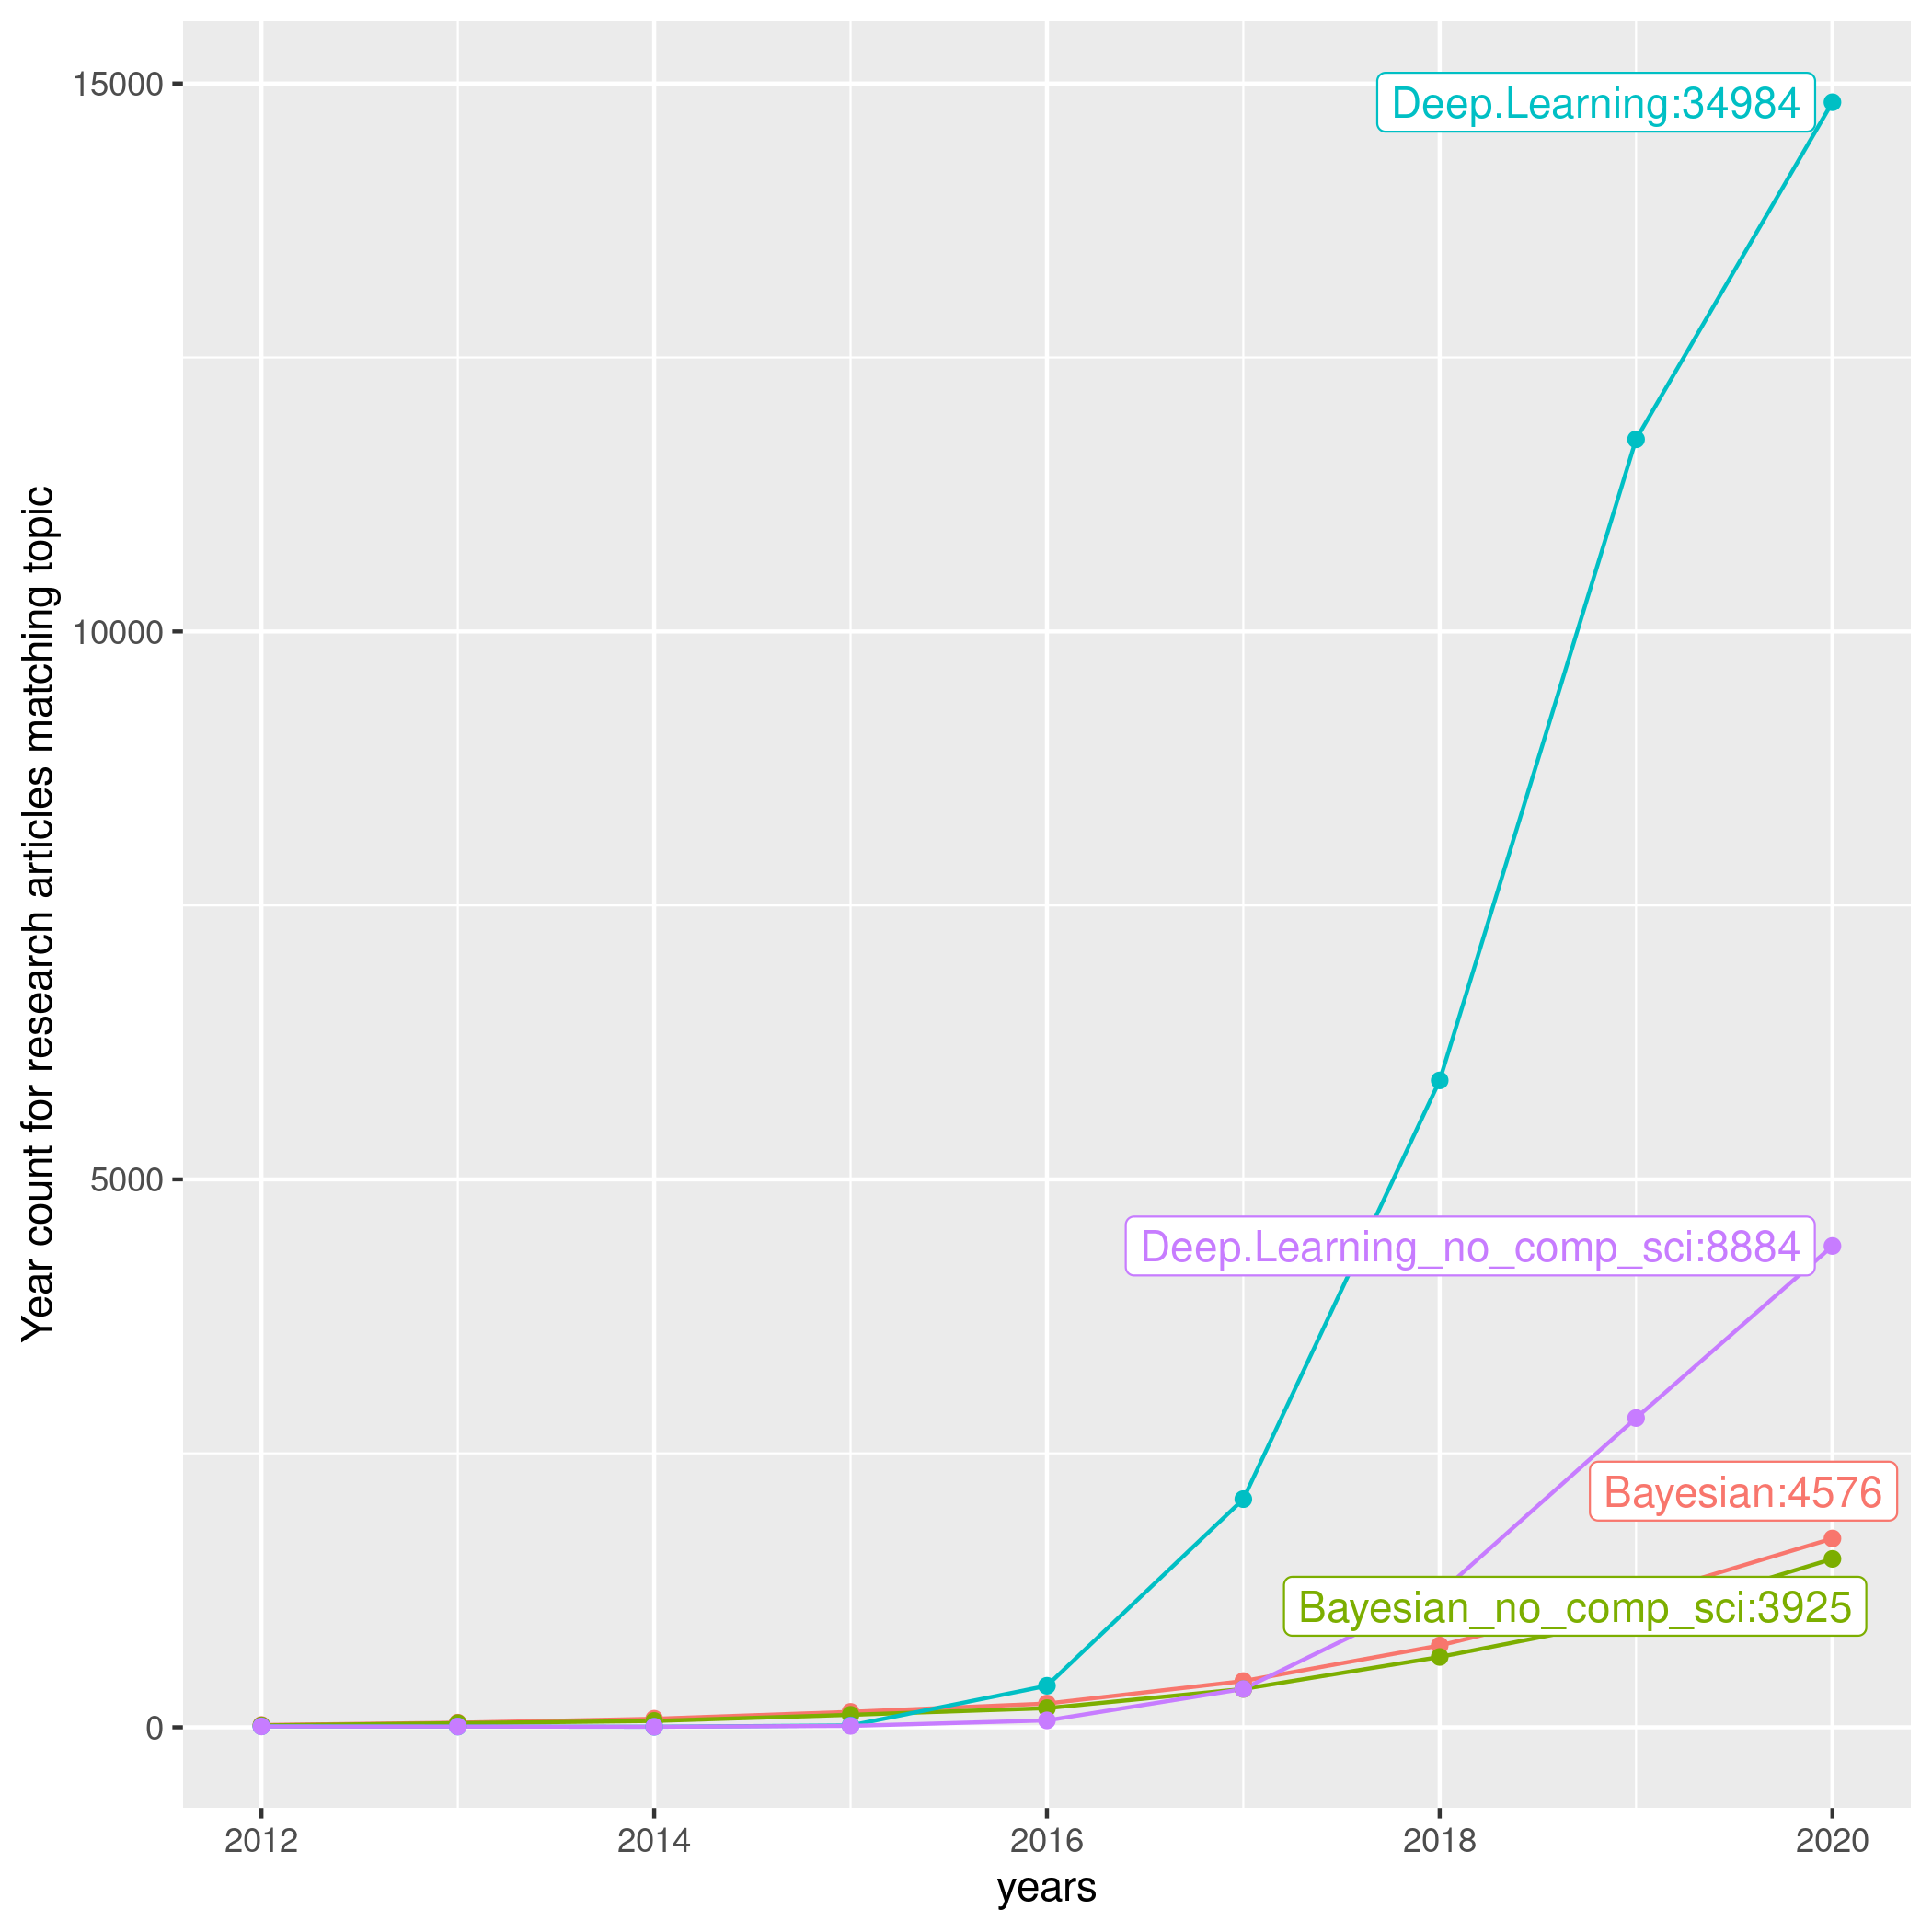
\includegraphics{CompSciVsNonCompSci}
\end{figure}



\end{document}
